%%%%%%%%%%%%%%%%%%%%%%%%%%%%%% -*- Mode: Latex -*- %%%%%%%%%%%%%%%%%%%%%%%%%%%%
%% uhtest.tex -- 
%% Author          : Robert Brewer
%% Created On      : Wed Sep 30 16:08:49 1998
%% Last Modified By: Robert Brewer
%% Last Modified On: Mon Oct  5 16:17:16 1998
%% RCS: $Id: uhtest.tex,v 1.2 1998/10/06 02:04:56 rbrewer Exp rbrewer $
%%%%%%%%%%%%%%%%%%%%%%%%%%%%%%%%%%%%%%%%%%%%%%%%%%%%%%%%%%%%%%%%%%%%%%%%%%%%%%%
%%   Copyright (C) 1998 Robert Brewer
%%%%%%%%%%%%%%%%%%%%%%%%%%%%%%%%%%%%%%%%%%%%%%%%%%%%%%%%%%%%%%%%%%%%%%%%%%%%%%%

%!!!!!!!!!!!!!!!!!!!!!!!!!!!!!!!!!!!!!!!!!!!!!!!!!!!!!!!!!!!!!!!!!!!!!!!!!!!!!!
%!NOTE: This example file has been prepared according to the University of
%!      Hawaii Style & Policy Manual for Theses and Dissertations dated
%!      "Revised February 1998". If you have one with a later date, you may
%!      need to make revisions to this document as well. In any event, making
%!      sure your thesis complies with Graduate Division guidelines is
%!      ultimately your responsibility. Caveat LaTeXtor. :)
%!!!!!!!!!!!!!!!!!!!!!!!!!!!!!!!!!!!!!!!!!!!!!!!!!!!!!!!!!!!!!!!!!!!!!!!!!!!!!!

%% The options are (you can only choose one from each group):
%%
%% 10pt, 11pt, 12pt: chooses the point size for the document. "11ot" is the
%%                   default.
%%
%% oneside, twoside: whether you want your document onesided or twosided. Note
%%                   that twosided is not guaranteed to work, and style
%%                   guidelines prohibit double sided printouts on final
%%                   copy. "oneside" is the default.
%%
%% draft, final: when printing drafts you can save a lot of paper by using the
%%               "draft" option. It switches to single spacing, displays overful
%%               hboxes with a black box, prints a version number on title page 
%%               and omits signature page. Of course for the final copy make
%%               sure to use the "final" option! "final" is the default.
%%
%% cm, times, palatino, newcent, bookman: switches between different font
%%                                        sets. "cm" is the Computer Modern
%%                                        font (TeX's default), the rest are
%%                                        PostScript fonts. "times" is the
%%                                        default.
%%
%% thesis, dissertation: switches between the style for a master's thesis and a 
%%                       Ph.D. dissertation. The differences are fairly minor
%%                       and limited to the front matter. "thesis" is the
%%                       default.
%%
%% actual, proposal: switches between actual document and proposal mode. In
%%                   proposal mode: the title page is simplified, the
%%                   version number is always printed, and the signature page
%%                   is omitted.
%%
%%% Load the uhthesis2e document class
\documentclass[11pt]{uhthesis2e}

%%% Load some useful packages:
%% New LaTeX2e graphics support
\usepackage{graphicx}
%% Package to linebreak URLs in a sane manner.
\usepackage{url}

%%% End of preamble
\begin{document}

%%% Declarations for Front Matter. Capitalize all of these values
%%% "normally". This allows the document class to format them properly.
%% Full title of thesis or dissertation, capitalized like a title should be.
\title{The Elements of Theses}
%% Your name, capitalized normally. Do not include any titles like Dr.
\author{Perry H. Disdainful}
%% Month in which you intend to receive your degree (i.e. graduation).
%% Presumably this will be one of: May, August, or December.
\degreemonth{May}
%% Year of expected graduation.
\degreeyear{2000}
%% Type of degree to be conferred.
\degree{Master of Science}
%% This is the chairperson of your committee. Do not use titles like Dr.
\chair{Rap Replinger}
%% The other members of your committee, seperated by "\\". Again, no titles,
%% and it is customary to list the outside committee member (if you have one)
%% last.
\othermembers{Andy Bumatai\\
Frank DeLima\\
Joseph B. Bogus}
%% This is the total size of your committee, including the chairperson. The
%% signature page routine will only handle up to 6 members; if you have more
%% than that you will need to modify the document class.
\numberofmembers{4}
%% The field in which you are obtaining your degree, capitalized normally.
\field{Information and Computer Sciences}
%% The version number of your document. Consistent use of this will enable you
%% to tell old drafts from new ones. Final actual documents omit this
%% automatically so you can use it without fear of submission problems at the
%% end. If you do not define this parameter, it defaults to "1.0.0".
\versionnum{2.1.1}

%%% Create the title page from all the information above. Note that the
%%% titlepage is outside the front matter.
\maketitle

\begin{frontmatter}

%%% Create the signature page (when indicated by the options)
\signaturepage

%%% Create the copyright page
\copyrightpage

%%% Bring in the dedication page from external file
%%%%%%%%%%%%%%%%%%%%%%%%%%%%%% -*- Mode: Latex -*- %%%%%%%%%%%%%%%%%%%%%%%%%%%%
%% uhtest-dedication.tex -- 
%% Author          : Robert Brewer
%% Created On      : Fri Oct  2 16:29:01 1998
%% Last Modified By: Robert Brewer
%% Last Modified On: Fri Oct  2 16:29:20 1998
%% RCS: $Id: uhtest-dedication.tex,v 1.1 1998/10/06 02:07:25 rbrewer Exp $
%%%%%%%%%%%%%%%%%%%%%%%%%%%%%%%%%%%%%%%%%%%%%%%%%%%%%%%%%%%%%%%%%%%%%%%%%%%%%%%
%%   Copyright (C) 1998 Robert Brewer
%%%%%%%%%%%%%%%%%%%%%%%%%%%%%%%%%%%%%%%%%%%%%%%%%%%%%%%%%%%%%%%%%%%%%%%%%%%%%%%
%% 

\begin{dedication}
\null\vfil
{\large
\begin{center}
To myself,\\\vspace{12pt}
Perry H. Disdainful,\\\vspace{12pt}
the only person worthy of my company.
\end{center}}
\vfil\null
\end{dedication}


%%% Bring in the acknowledgments section from external file
%%%%%%%%%%%%%%%%%%%%%%%%%%%%%% -*- Mode: Latex -*- %%%%%%%%%%%%%%%%%%%%%%%%%%%%
%% uhtest-acknowledgements.tex -- 
%% Author          : Robert Brewer
%% Created On      : Fri Oct  2 16:29:43 1998
%% Last Modified By: Robert Brewer
%% Last Modified On: Fri Oct  2 16:29:52 1998
%% RCS: $Id: uhtest-acknowledgements.tex,v 1.1 1998/10/06 02:06:54 rbrewer Exp $
%%%%%%%%%%%%%%%%%%%%%%%%%%%%%%%%%%%%%%%%%%%%%%%%%%%%%%%%%%%%%%%%%%%%%%%%%%%%%%%
%%   Copyright (C) 1998 Robert Brewer
%%%%%%%%%%%%%%%%%%%%%%%%%%%%%%%%%%%%%%%%%%%%%%%%%%%%%%%%%%%%%%%%%%%%%%%%%%%%%%%
%% 

\begin{acknowledgments}
I want to ``thank'' my committee, without whose ridiculous demands, I
would have graduated so, so, very much faster.
\end{acknowledgments}


%%% Bring in the abstract section from external file
%%%%%%%%%%%%%%%%%%%%%%%%%%%%%% -*- Mode: Latex -*- %%%%%%%%%%%%%%%%%%%%%%%%%%%%
%% uhtest-abstract.tex -- 
%% Author          : Robert Brewer
%% Created On      : Fri Oct  2 16:30:18 1998
%% Last Modified By: Robert Brewer
%% Last Modified On: Fri Oct  2 16:30:25 1998
%% RCS: $Id: uhtest-abstract.tex,v 1.1 1998/10/06 02:06:30 rbrewer Exp $
%%%%%%%%%%%%%%%%%%%%%%%%%%%%%%%%%%%%%%%%%%%%%%%%%%%%%%%%%%%%%%%%%%%%%%%%%%%%%%%
%%   Copyright (C) 1998 Robert Brewer
%%%%%%%%%%%%%%%%%%%%%%%%%%%%%%%%%%%%%%%%%%%%%%%%%%%%%%%%%%%%%%%%%%%%%%%%%%%%%%%
%% 

\begin{abstract}
Theses have elements.  Isn't that nice?

\end{abstract}


%%% Generate table of contents
\tableofcontents

%%% Generate list of tables
\listoftables

%%% Generate list of figures
\listoffigures

\end{frontmatter}

%%% Bring in the body of the thesis from external file
%%%%%%%%%%%%%%%%%%%%%%%%%%%%%% -*- Mode: Latex -*- %%%%%%%%%%%%%%%%%%%%%%%%%%%%
%% uhtest-body.tex -- 
%% Author          : Robert Brewer
%% Created On      : Fri Oct  2 16:30:37 1998
%% Last Modified By: Robert Brewer
%% Last Modified On: Mon Oct  5 16:01:29 1998
%% RCS: $Id: uhtest-body.tex,v 1.1 1998/10/06 02:07:14 rbrewer Exp $
%%%%%%%%%%%%%%%%%%%%%%%%%%%%%%%%%%%%%%%%%%%%%%%%%%%%%%%%%%%%%%%%%%%%%%%%%%%%%%%
%%   Copyright (C) 1998 Robert Brewer
%%%%%%%%%%%%%%%%%%%%%%%%%%%%%%%%%%%%%%%%%%%%%%%%%%%%%%%%%%%%%%%%%%%%%%%%%%%%%%%
%% 

\chapter{Introduction}

Every dissertation should have an introduction.  You might not realize
it, but the introduction should introduce the concepts, background,
and goals of the dissertation.

Examples of great literature can be found in table \ref{tab:example-1}.

%% Here is an example of how to create a floating table. Note that the caption
%% occurs _before_ the table, unlike a figure where it appears after!
%%
%% The "[htbp]" allows the table to be placed: here, top of page, bottom of
%% page or on a seperate floats page, whatever works best.
\begin{table}[htbp]
  %% If you have a really long caption, you can enclose a short version for the
  %% the List of Tables in "[]", and the full caption in "{}" as we do here
  \caption[A normal size table.]{A normal size table. There has been a complaint
    that table captions are not single-spaced, but they should be. This is a
    test of that feature.}
  %% This label allows references from other parts of the text to be
  %% automatically calculated. Labels usually start with three letters
  %% describing what is being tabled followed by a colon. This prevents label
  %% mixups. Note that the label must follow the caption for proper numbering.
  \label{tab:example-1}
  \begin{center}
    \begin{tabular}{|l|r|}
      \hline 
      Title & Author \\
      \hline
      War And Peace & Leo Tolstoy \\
      The Great Gatsby & F. Scott Fitzgerald \\ \hline
    \end{tabular}
  \end{center}
\end{table}

For an example of a smaller size table, see table \ref{tab:example-2}.

\begin{table}[htbp]
  \caption{A small table.}
  \label{tab:example-2}
  \begin{center}
    \begin{scriptsizetabular}{|l|r|}
      \hline 
      Title & Author \\
      \hline
      War And Peace & Leo Tolstoy \\
      The Great Gatsby & F. Scott Fitzgerald \\ \hline
    \end{scriptsizetabular}
  \end{center}
\end{table}

\chapter{Previous Work}

Some other research was once performed. You can check out a beautiful picture
in figure \ref{fig:example-1}.

\begin{figure}[htbp]
  \centering
  \includegraphics{uhtest-figure.eps}
  \caption{An example of included Encapsulated PostScript (EPS).}
  \label{fig:example-1}
\end{figure}

\section{URLs}
In this modern age, you may find that you wish to include URLs or pathnames
which both tend to be long and hard for TeX to deal with because it doesn't
know where to insert linebreaks. The ``{\tt url}'' package (loaded in the main
uhtest.tex file) allows one to deal with these URLs. For example:

Here is an URL which cannot be broken, leading to terrible output
$<$http://www.hotwired.com/webmonkey/98/16/index2a.html$>$
%% The "<>" have to be entered in math mode, that's where the "$"s come from.

Using the package we get the much nicer \url{<http://www.hotwired.com/
webmonkey/98/16/index2a.html>} which LaTeX can handle just fine. Even better,
the parameter to {\tt $\backslash$url} can have spaces inserted anywhere so you
can make the LaTeX source lines in your text editor wrap nicely.

A few notes. It is recommended that you enclose your URLs in ``$<>$'' to ensure
that any punctuation around the URL won't be confused as part of the URL. You
can use URLs in your bibliography too (see the {\tt uhtest.bib} file for an
example). Finally, if you need to use a tilde in your URL then things are a
little trickier. One way to do it is like this:
\url{<http://www.dartmouth.edu/}$\sim$\url{jonh/ff-cache/1.html>}. The {\tt
$\backslash$url} style uses math mode internally, so we break the URL into two
pieces, and stick a tilde from math mode inbetween the two parts.

\section{Bibliography Citations}
Citing references to your bibliography is easy \cite{lamport:latex}
\cite{patashnik:bibtex}. First you build a BibTeX file which contains the
records for all of the works you wish to cite. This file ends with a ``{\tt
.bib}'' extension. Then in your body you use the ``{\tt $\backslash$cite}''
command with the label you gave to the record in question. The final steps are: 
run LaTeX once, run BibTeX, and then run LaTeX twice more. You should now have
a bibliography that includes those citations.

\chapter{Conclusion}

This is going to be the chapter where I check the length of the page to make
sure the bottom margin works out all right.  I hope you don't mind long
annoying and useless paragraphs because you are sure to get a lot of them here!

\section{Widgets}

This is going to be the chapter where I check the length of the page
to make sure the bottom margin works out all right.  I hope you don't
mind long annoying and useless paragraphs because you are sure to get
a lot of them here!

\subsection{Sub-Widgets}

This is going to be the chapter where I check the length of the page
to make sure the bottom margin works out all right.  I hope you don't
mind long annoying and useless paragraphs because you are sure to get
a lot of them here!

\subsubsection{Sub-Sub-Widgets}

This is going to be the chapter where I check the length of the page
to make sure the bottom margin works out all right.  I hope you don't
mind long annoying and useless paragraphs because you are sure to get
a lot of them here!

\paragraph{Para-Widgets}

This is going to be the chapter where I check the length of the page
to make sure the bottom margin works out all right.  I hope you don't
mind long annoying and useless paragraphs because you are sure to get
a lot of them here!

\subparagraph{Sub-Para-Widgets}

This is going to be the chapter where I check the length of the page
to make sure the bottom margin works out all right.  I hope you don't
mind long annoying and useless paragraphs because you are sure to get
a lot of them here!

This is going to be the chapter where I check the length of the page
to make sure the bottom margin works out all right.  I hope you don't
mind long annoying and useless paragraphs because you are sure to get
a lot of them here!

This is going to be the chapter where I check the length of the page
to make sure the bottom margin works out all right.  I hope you don't
mind long annoying and useless paragraphs because you are sure to get
a lot of them here!

This is going to be the chapter where I check the length of the page
to make sure the bottom margin works out all right.  I hope you don't
mind long annoying and useless paragraphs because you are sure to get
a lot of them here!

This is going to be the chapter where I check the length of the page
to make sure the bottom margin works out all right.  I hope you don't
mind long annoying and useless paragraphs because you are sure to get
a lot of them here!

This is going to be the chapter where I check the length of the page
to make sure the bottom margin works out all right.  I hope you don't
mind long annoying and useless paragraphs because you are sure to get
a lot of them here!

This is going to be the chapter where I check the length of the page
to make sure the bottom margin works out all right.  I hope you don't
mind long annoying and useless paragraphs because you are sure to get
a lot of them here!

This is going to be the chapter where I check the length of the page
to make sure the bottom margin works out all right.  I hope you don't
mind long annoying and useless paragraphs because you are sure to get
a lot of them here!

This is going to be the chapter where I check the length of the page
to make sure the bottom margin works out all right.  I hope you don't
mind long annoying and useless paragraphs because you are sure to get
a lot of them here!

This is going to be the chapter where I check the length of the page
to make sure the bottom margin works out all right.  I hope you don't
mind long annoying and useless paragraphs because you are sure to get
a lot of them here!

This is going to be the chapter where I check the length of the page
to make sure the bottom margin works out all right.  I hope you don't
mind long annoying and useless paragraphs because you are sure to get
a lot of them here!

This is going to be the chapter where I check the length of the page
to make sure the bottom margin works out all right.  I hope you don't
mind long annoying and useless paragraphs because you are sure to get
a lot of them here!

This is going to be the chapter where I check the length of the page
to make sure the bottom margin works out all right.  I hope you don't
mind long annoying and useless paragraphs because you are sure to get
a lot of them here!

This is going to be the chapter where I check the length of the page
to make sure the bottom margin works out all right.  I hope you don't
mind long annoying and useless paragraphs because you are sure to get
a lot of them here!

This is going to be the chapter where I check the length of the page
to make sure the bottom margin works out all right.  I hope you don't
mind long annoying and useless paragraphs because you are sure to get
a lot of them here!

This is going to be the chapter where I check the length of the page
to make sure the bottom margin works out all right.  I hope you don't
mind long annoying and useless paragraphs because you are sure to get
a lot of them here!


%%% Bring in any appendices from external file
%%%%%%%%%%%%%%%%%%%%%%%%%%%%%% -*- Mode: Latex -*- %%%%%%%%%%%%%%%%%%%%%%%%%%%%
%% uhtest-appendix.tex -- 
%% Author          : Robert Brewer
%% Created On      : Fri Oct  2 16:31:12 1998
%% Last Modified By: Robert Brewer
%% Last Modified On: Mon Oct  5 14:41:05 1998
%% RCS: $Id: uhtest-appendix.tex,v 1.1 1998/10/06 02:07:03 rbrewer Exp $
%%%%%%%%%%%%%%%%%%%%%%%%%%%%%%%%%%%%%%%%%%%%%%%%%%%%%%%%%%%%%%%%%%%%%%%%%%%%%%%
%%   Copyright (C) 1998 Robert Brewer
%%%%%%%%%%%%%%%%%%%%%%%%%%%%%%%%%%%%%%%%%%%%%%%%%%%%%%%%%%%%%%%%%%%%%%%%%%%%%%%
%% 

\appendix
\chapter{Some Ancillary Stuff}

Ancillary material should be put in appendices, which appear before the
bibliography. 

\chapter{More Ancillary Stuff}

Subsequent chapters are labeled with letters of the alphabet.


%% Just for demo purposes, include all entries from bib file
\nocite{*}

%%% Input file for bibliography
\bibliography{uhtest}
%% Use this for an alphabetically organized bibliography
\bibliographystyle{plain}
%% Use this for a reference order organized bibliography
%\bibliographystyle{unsrt}

\end{document}
